\graphicspath{{chapters/11/images}}
\chapter{Stochastic methods for parameter estimation}

\section{Introduction}
Stochastic methods are often used when we cannot compute the gradient.
With the same parameters, stochastic methods can produce dramatically different results, as it can be seen in figure \ref{fig:res}.

\begin{figure}[H]
  \centering
  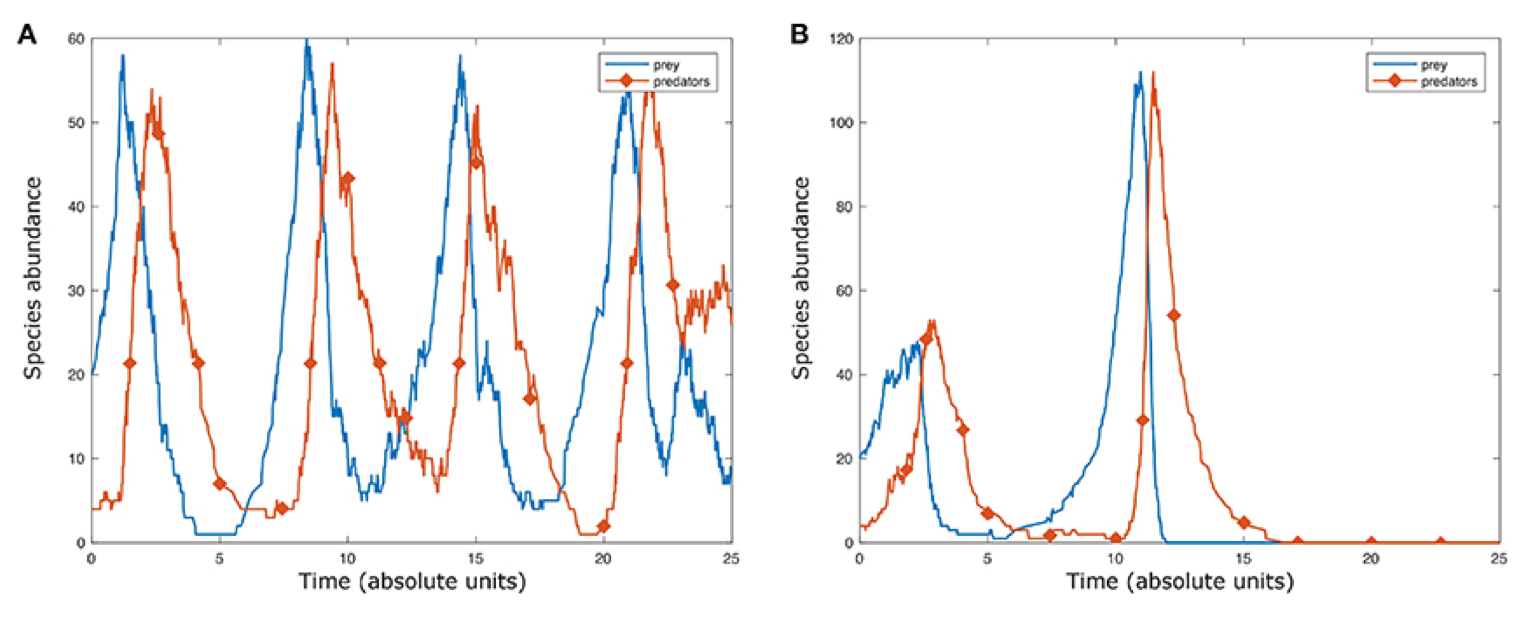
\includegraphics[width=\textwidth]{stoch_LV.png}
  \caption{Lotka-Volterra stochastic simulation results. In B we witness
  preys and predators extinction, it is the output of a simulation
  performed with the same model and parameters as A.}
\label{fig:res}
\end{figure}

Instead of following the gradient informations are collected in a manner resembling natural selection.
Monte Carlo Methods are dated around 1949, the name comes from casinos.
In order to use MCM to do inference, Metropoli and Hastings developed a specific algorithm in 1970.

\section{Markov Chain Monte Carlo (MCMC)}
MCMC is a chain of events where the current state depends on the previous one and on the transition probability.
Running MCMC long enough they will reach a stable point.
$x^{(i)}$ is a random variable or stochastic process that takes only discrete values $\{x_1,\dots,x_s\}$.
Let $p(x)$ be the probability distribution of $x$.

  \subsection{Markov chain}
  $x^{(i)}$ is a Markov Chain if:

  $$p(x^{(i)}|x^{(i-1)},\dots,x^{(1)})=T(x^{(i)}|x^{(i-1)})$$

    \subsubsection{Homogeneity}
    A Markov chain is homogenous if $T(x^{(i)})x^{(i-1)}=T$,
    So that the transition matrix is constant.

  \subsection{Example}
  Let $3$ states as in figure \ref{fig:MCMCexmple}.

  \begin{figure}
    \centering
    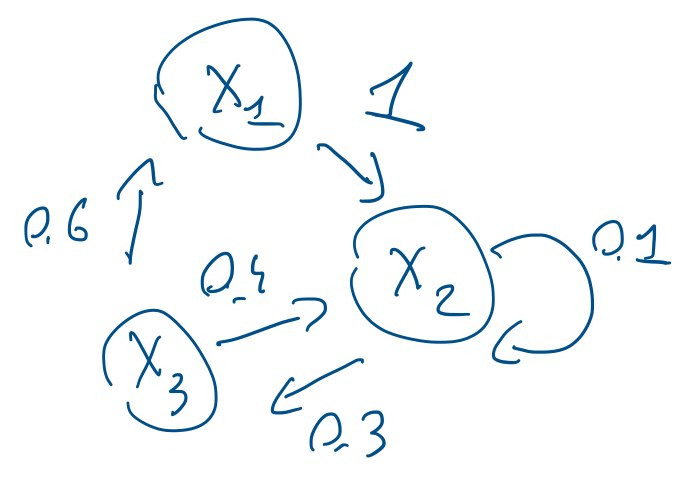
\includegraphics[width=0.3\textwidth]{mcmc.png}
    \caption{MCMC example}
    \label{fig:MCMCexample}
  \end{figure}

  The homogeneous transition matrix:

  $$T = \begin{bmatrix}0 & 1 & 0\\0 & 0.1 & 0.9\\ 0.6 & 0.4 & 0\\\end{bmatrix}$$

  And the states:

  $$\pi_1=\begin{pmatrix}0.5 & 0.2& 0.3 \end{pmatrix}$$

  The next probability of being in the three states is given by

  $$\pi_1 \cdot T=\begin{pmatrix}0.3\cdot0.6, & 0.5+0.02+0.12,& 0.18 \end{pmatrix} = \begin{pmatrix}0.18, & 0.64,& 0.18 \end{pmatrix}$$

  Iterating enough time a fixed distribution will be reached.

  \subsection{Invariant distribution}
  The invariant distribution if a fixed distribution reached after enough Monte Carlo iterations.
  The objective is to build a Markov chain whose invariant distribution is the distribution of the unknown parameters.
  For example, in the previous example, the invariant distribution will be:

  $$p(x)=\dots = \begin{pmatrix} 0.2213 \\ 0.4098 \\ 0.3689\end{pmatrix}^T$$

  \subsection{Irreducible matrices}
  A stochastic matrix is irreducible if its graph does not contain unconnected sub-graphs.
  If $T$ is an irreducible transition matrix and is aperiodic the Markov chain has an invariant distribution.
  The probability distribution has to be linked with the model.

  \subsection{Monte Carlo sampling}
  Monte Carlo refers to a family of methods developed for sampling.
  In particular, the output of a Monte Carlo method are independent and identically distributed random variables $\{x^{(i)}\}_{i>0}$ from a known density $p(X)$.
  The samples can be used to ``estimate or approximate'' a target density or distribution.
  Known distributions are exploited to approximate the unknown distribution of interest.
  Given enough samples, $p$ can be approximated as:

  $$p_N(x)= \frac{1}{N}\sum^N_{i=1}\delta_{x^{(i)}}(x)$$

  With:

  $$\delta_{x^{(i)}}(x)= \begin{cases}1, & x=x^{(i)} \\ 0, & \text{elsewhere}\end{cases}$$

  This is often used to approximate ``hard'' integrals.
  An integral with a finite sum of values, can be obtained as:

  $$I_N(f)=\frac{1}{N} \sum^N_{i=1} f(x^{(i)})$$

  The function is being evaluated as some points and the mean is an integration of the integral.
  This equation converges to the real integral by the law of large numbers:

  $$I_N(f)=\frac{1}{N} \sum^N_{i=1} f(x^{(i)})  \xrightarrow[N \rightarrow \infty  ]{}   I(f)= \int_x f(x)p(x)dx$$

  This is better than the output of the least square problem as it gives information about the shape of the distribution.

\section{Sampling a distribution}
Let $p$ be a known probability distribution up to a proportionality constant.
It is usually preferred to sample from a well-known distribution, like for example the one in \ref{fig:bimodal}.

$$q(x)\text{ such that }\exists M>0$$

$$p(x) \leq M q(x)$$


\begin{figure}
  \centering
  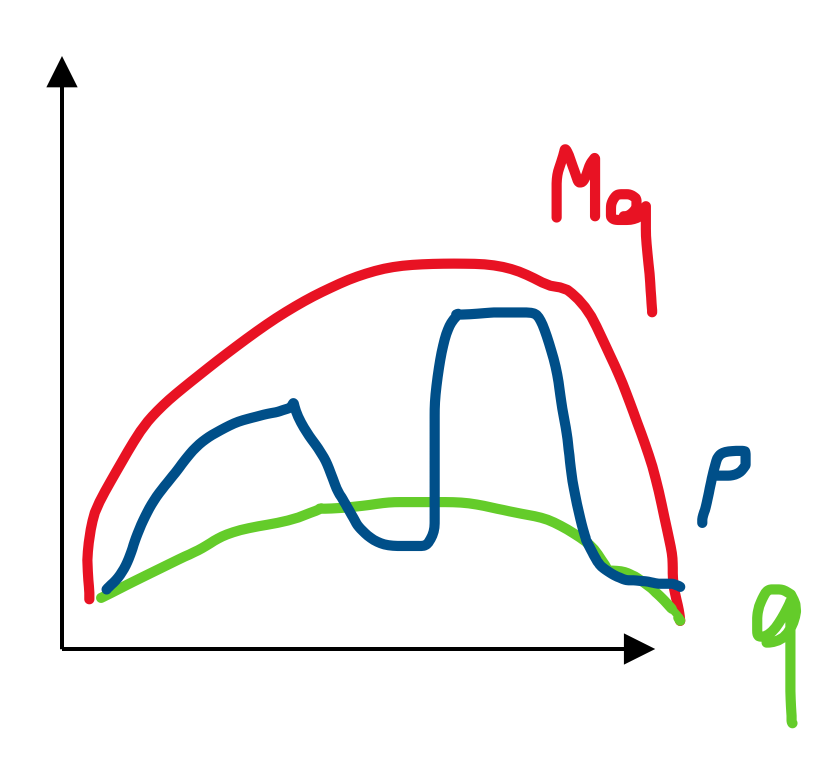
\includegraphics[width=0.3\textwidth]{distribution.png}
  \caption{Example: bimodal distribution}
  \label{fig:bimodal}
\end{figure}

Values from $q$ are extracted if they are smaller than $Mq$.
Each time information about $p$ are collected from $q$.

  \subsection{Rejection sampling algorithm}
  A rejection sampling implementation is outlined in algorithm \ref{algo:rejection-sampling}.

  \begin{algorithm}[H]
\DontPrintSemicolon
\SetKwComment{comment}{$\%$}{}
\SetKw{Int}{int}
\SetKw{To}{to}
\SetKw{Return}{return}
\SetKw{Not}{not}
\SetKw{Input}{Input}
\SetKw{Output}{Output}
\SetKw{False}{false}
\SetKw{True}{true}
\SetKwData{Item}{item}
\SetKwFunction{Min}{min}
\SetKwFunction{Partitioning}{partitioning}
\SetKwFunction{TitleFunction}{Rejection sampling}

\caption{\protect\TitleFunction{}}
\label{algo:rejection-sampling}

\Input: $M$, $p(x)$ and $q(x)$\;

\Output: a random variable distributed according to $p$\;

$i = 1$\;
\Repeat{}{
	sample $x^{(i)}\sim q$, $u\sim norm(0,1)$\;
	\If{$u>\frac{p(x^{(i)})}{Mq(X^i)}$}{
		$i = i + 1$\;
	}
}

\end{algorithm}


  If the point is in the area between $p$ and $Mq$ is accepted.
  The further the ratio is from $1$, the smaller the chance of keeping the point.
  A known distribution $p$ is being used, then gradually what is known about it is removed in the following iterations.

\section{Metropolis Hastings}
Let $X$ be the current point, $q$ the proposal distribution and $p$ the target distribution.
$p$ can be an unnormalized density ($\int p > 1 \text{ but} \int p < \infty)$.
Ideally $p$ should be known, but if it is not the procedure still works.
Let $h$ be the non negative and positive integral of the normalized density distribution.
The trick of MH is to avoid relying on the probability: a function is used instead.
Let $x*+^*$ be the new candidate point, then the metropolis ratio is defined as:

$$r_M(x,x^*)=\frac{h(x^*)}{h(x)}$$

And the Hasting ratio:

$$r_H(x,x^*)=\frac{h(x^*)\cdot q(x^*|x)}{h(x)\cdot q(x|x^*)}$$

From the distribution, the objective is to measure how likely the previous value is given the current one.
The choices is being weighted to the likeliness.

  \subsection{Algorithm}
  An implementation of the Metropolis Hastings method is outlined in algorithm \ref{algo:mh}

  
\begin{algorithm}[H]
\DontPrintSemicolon
\SetKwComment{comment}{$\%$}{}
\SetKw{Int}{int}
\SetKw{To}{to}
\SetKw{Return}{return}
\SetKw{Not}{not}
\SetKw{Input}{Input}
\SetKw{Output}{Output}
\SetKw{False}{false}
\SetKw{True}{true}
\SetKwData{Item}{item}
\SetKwFunction{Min}{min}
\SetKwFunction{Partitioning}{partitioning}
\SetKwFunction{TitleFunction}{Metropolis Hastings}

\caption{\protect\TitleFunction{}}
\label{algo:mh}

\Input: $N$, $r$ and $q(x)$\;

\Output: a random variable distributed according to $p$\;

guess $x^{(i)}$\;

\ForEach{$i = 0,\dots, N-1$}{
	sample $s^*\sim q(\cdot|x^{(i)})$ and $u\sim norm(0,1)$\;
	\If{$u<\min\{1, r_H(x,x^*)\}$}{
		$x^{(i+1)} = x^{(*)}$\;
	}
	\Else{
		$x^{(i+1)} = x^{(i)}$\;
	}
}

\end{algorithm}


  So in this algorithm the proposal distribution is sampled and the sample is accepted if it is more likely, if it is not it is accepted with a certain chance.


  \subsection{Visualization of MCMC}
  MATLAB plot:

  \begin{itemize}
  \tightlist
  \item
    right: histogram with the known distribution
  \item
    left: MCMC oscillating between 0 and 10, recapitulates the
    distribution
  \end{itemize}
  \noindent
  The procedure is really fast, takes less than a second. If instead of
  extracting u and v from random distribution with an index, the result is
  the same → ``thanks MATLAB, it is not necessary to prelocate anymore''
  \\
  \\
  \noindent
  If we employ a Gaussian distribution, the result is still good but not
  as accurate as the previous one. We are adding complexity by introducing
  the variance; by choosing a different value we can improve the result.
  Pay attention to the fact that if we sample from a narrow distribution,
  we risk focusing only on one of the two points.
  \\
  \\
  \noindent
  Everything we do has consequences!

  \url{http://chi-feng.github.io/mcmc-demo/app.html?algorithm=RandomWalkMH\&target=banana}
  \noindent
  Green: accept, red: reject
  \\
  \\
  \noindent
  \underline{Target distribution = standard}

  \begin{itemize}
  \tightlist
  \item
    GibbsSampling: collects points according to a certain direction from a
    starting point, it tries to rebuild a 2D Normal distribution.
  \item
    AdaptiveMH: sample from a starting mean and accept or reject new
    points.
  \item
    Random walk: more or less like MH. Even if the target distribution is
    not that difficult (bell shape), there are a lot of rejections
    initially.
  \item
    DE-MCMC-Z: produces vectors.
  \end{itemize}
  \noindent
  \underline{Target distribution = donut}

  \begin{itemize}
  \tightlist
  \item
    SVGO: stochastic vector gradient descent, intermediate between
    gradient and stochastic.
  \item
    EfficientNUTS (No-U-Turn samples): it creates many points, more
    complex but one of the best. In the end it will converge quite fast.
  \item
    RandomWalk: needs more time to converge with respect to standard
    distribution.
  \end{itemize}
  \noindent
  \underline{Target distribution = multimodal}

  \begin{itemize}
  \tightlist
  \item
    RandomWalk: three initial points, it proposes a random perturbation.
  \item
    AdaptiveMH: changes some of the parameters. Differently from the
    previous approach, the shape changes: instead of having a fixed search
    area, it evolves and adapts.
  \end{itemize}


\section{How to link data and MH}
In least square methods, the function that was used was:

$$f(\theta)=\frac{1}{2}\sum^m_{j=1}r^2_j(\theta)=\frac{1}{2}\sum^m_{j=1}(y_j-m_j(t_i,\theta))^2$$

The residuals can be weighted for their uncertainty:

$$f_w(\theta)=\frac{1}{2}\sum^m_{j=1} \frac{r^2_j(\theta)}{\vartheta_j^2}$$

$\vartheta_j$ can be, for example, the standard deviation of that measured point.
Let $Y$ be the vector of observations, a function that can be used to link the parameters and the output can be the non negative:

$$L(\theta|Y)=\exp(-f_w(\theta)) \geq 0$$

This can be used as the $h$ in the MH algorithm, so that the Metropolis ratio:

$$r_H(\theta^*,\theta)=\frac{L(\theta^*)}{L(\theta)}=\frac{e^{-f_w(\theta^*)}}{e^{-f_w(\theta)}}=\exp(-f_w(\theta^*)+-f_w(\theta))$$

Since $f_w(\theta)\geq0$, if $f_w(\theta^*) > f_w(\theta) \Rightarrow r_H>1$ , the number is accepted, otherwise it is accepted according to a certain probability.
This function can be used to link new parameters with data.
Another example of this type of function is the log-likelihood, considering:

$$f_w(\theta^*)\qquad\land\qquad f_w(\theta)$$


\section{Random walk MCMC}
Assume that $\theta^*$ is sampled from:

$$\mathcal{N}(0,\mathcal{C})+\theta=\mathcal{N}(\theta,\mathcal{C})$$

Now a perturbation is added with $\mathcal{C}$, the covariance matrix, which can be fixed or adapted along the iterations.
From the initial point there is a new candidate according to a multivariate normal distribution.
If the candidate is accepted, the evaluation is restarted from it.
This allows to collect informations about the shape of the target distribution.


  \subsection{Algorithm RW-MCMC ( C known)}
  An implementation of the RW-MCMC is oulined in algorithm \ref{algo:rw-mcmc}.

  \begin{algorithm}[H]
\DontPrintSemicolon
\SetKwComment{comment}{$\%$}{}
\SetKw{Int}{int}
\SetKw{To}{to}
\SetKw{Return}{return}
\SetKw{Not}{not}
\SetKw{Input}{Input}
\SetKw{Output}{Output}
\SetKw{False}{false}
\SetKw{True}{true}
\SetKwData{Item}{item}
\SetKwFunction{Min}{min}
\SetKwFunction{Partitioning}{partitioning}
\SetKwFunction{TitleFunction}{Random walk Markov Chain Monte Carlo (RW-MCMC)}

\caption{\protect\TitleFunction{}}
\label{algo:rw-mcmc}

\Input: $L$, $\theta$\;

\Output: a random variable distributed according to $p$\;

initialize matrix $D_\theta$ and vector $V_L$\;
generate randomly $\theta_1$\;
$L(\theta_1) = L_1$\;
\ForEach{$i = 1, \dots, N$}{
	$Z\sim norm(D, \mathcal{C})$\;
	$\theta_2$ = $\theta_1 +Z$\;
	$L_2 = L(\theta_2)$\;
	$ratio = \frac{L_1}{L_2}$\;
	$u\sim norm(0,1)$\;
	\If{$u<ratio$}{
		$L_1 = L_2$\;
		$\theta_1 = \theta_2$\;
	}
	\If{$i>warm\_up$}{
		$D_\theta = [D_\theta;\theta_1]$\;
		$V_L = [V_L;L_1]$\;
	}
}
\end{algorithm}


  \subsection{Discussion}
  To reach a satisfactory convergence a good accept-reject tradeoff should be obtained.
  The advantages of RW-MCMC are:

  \begin{multicols}{2}
    \begin{itemize}
      \item The object function is evaluated once per iteration.
      \item The target distribution can be built form the samples.
      \item Only the last point is necessary for the algorithm.
      \item Info on the model can be collected: the variability on the output and the sensitivity on parameters.
      \item Random selection helps to avoid local minima.
    \end{itemize}
  \end{multicols}

  The disadvantages of RW-MCMC are:

  \begin{multicols}{2}
    \begin{itemize}
      \item Convergence may be slow.
      \item The sampling distribution may affect the results.
      \item Each MCMC cannot be parallelized.
      \item Burn-time.
      \item Diagnostics are heuristics.
    \end{itemize}
  \end{multicols}]

  \subsection{Diagnostics}
  Diagnostics are used to checked the goodness of the parameters and whether the iterations have finished.
  Consider for example figure \ref{fig:dia-1}:

  \begin{multicols}{2}
    \begin{itemize}
      \item chain 1: expected MCMC plot.
      \item chain 2: requires a longer burn-in, as the target distribution has not been reached.
      \item chain 3: there aren't enough information because the number of iterations is too small.
    \end{itemize}
  \end{multicols}

  \begin{figure}[H]
    \centering
    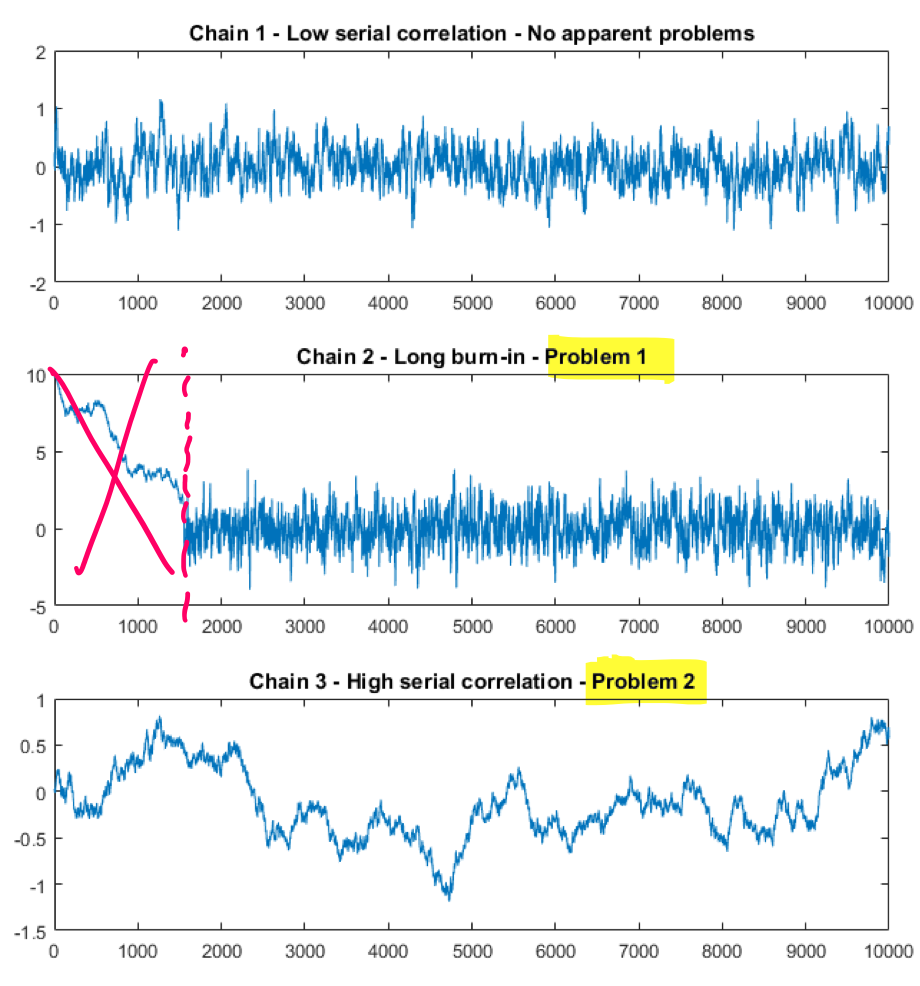
\includegraphics[width=0.5\textwidth]{diag_1.png}
    \caption{Diagnostic 1}
    \label{fig:dia-1}
  \end{figure}

  The desired output of MCMC should look like the plots in figure \ref{fig:dia-2}.

  \begin{figure}[H]
    \centering
    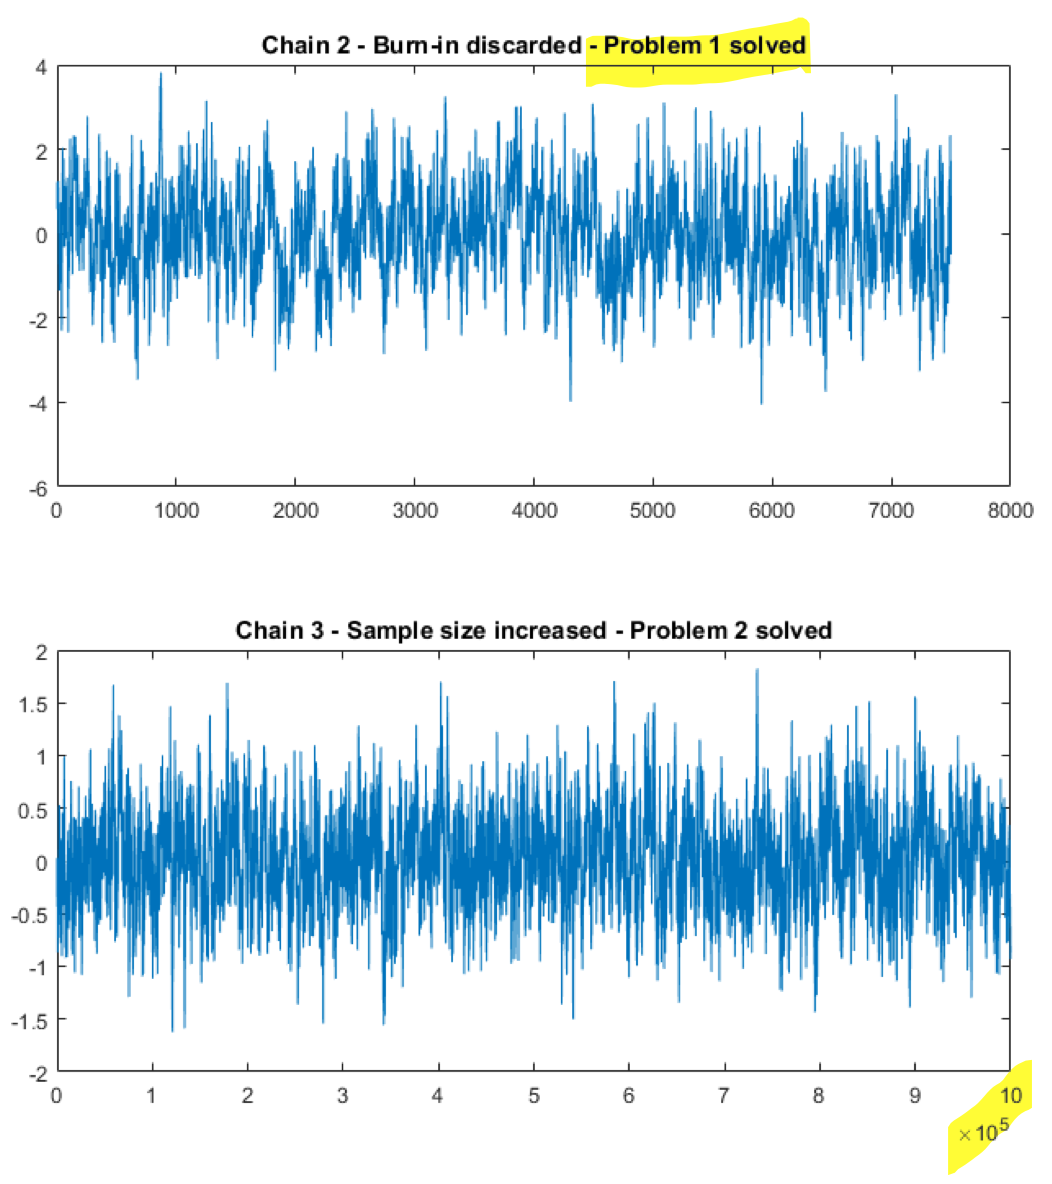
\includegraphics[width=0.5\textwidth]{diag_2.png}
    \caption{Diagnostic 2}
    \label{fig:dia-2}
  \end{figure}


    \subsubsection{Sample split}
    Sample split is a more analytical approach in which the plots are split in different regions and it is checked whether the sub-regions have the same mean.
    It can be seen in figure \ref{fig:dia-3} there is no longer a need for warm-up in the second plot, while in the third more samples are still needed.

    \begin{figure}
      \centering
      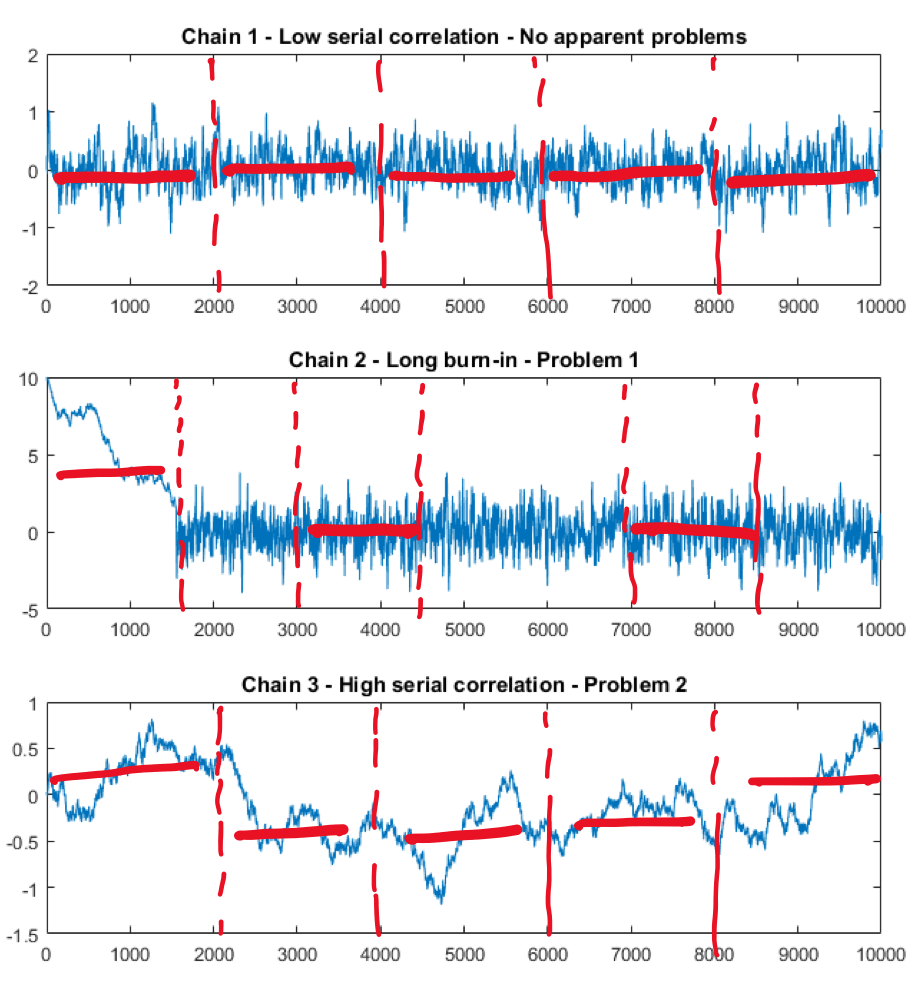
\includegraphics[width=0.5\textwidth]{diag_3.png}
      \caption{Diagnostic 3}
      \label{fig:dia-3}
    \end{figure}

    \subsubsection{Conclusions}
    Differently from gradient methods, here things are a bit more hard to interpret.
    Eventually oscillations around the global optimum will be reached, but there is no guarantee.
    Diagnostics are based on the observation of the results, so they might
    be biased by the observers' believes and they do not provide an easy way to read a ``certificate'' of convergence.
    Another approach may be to run more MCMC in parallel and see if they all converge to the same distribution.
    However, it is again not a certificate of convergence to the global optimum.
    Constraints and bounds can be included easily in the proposal distribution or in the likelihood.
